\section{How Fast the Offloaded Stack Runs}\label{sec:results}\label{sec:results-controlled}

This section measures the speed of the offloaded stack: how long users wait, how fast replies are written, and how
both change with load, prompt length, the share of experts on the host and the host itself. It cannot say how much
of any slowdown the offload causes, because the reference with everything in GPU memory (E9) did not run. Only the two
host shares of E3 isolate part of that cost (Section~\ref{sec:limits}).

\paragraph{Reading and writing.}
One distinction makes the rest of the section easy to follow. Serving a request has two phases. In the first the model
\emph{reads} the prompt. It processes every prompt token in one pass, which is limited by compute and grows with the
prompt's length. In the second it \emph{writes} the reply one token at a time, and each step must fetch the weights of
the experts the router picks for that token, which is limited by memory traffic, including the reads from the back
room. vLLM~\citep{kwon2023vllm} keeps the KV cache in pages, batches requests continuously and splits long prompts into
chunks that share steps with ongoing replies~\citep{agrawal2024sarathi}. It also caches prompt prefixes, so a request
that shares a prefix with an earlier one skips reading it~\citep{zheng2024sglang,vllm2026prefixcaching}. Two numbers
follow from the two phases. The \emph{time to first token} (TTFT) is how long a user waits before anything appears,
which is mostly reading. The \emph{time per output token} (TPOT) is the pace of writing, and its inverse, the rate per
stream in tokens/s, is what a user perceives as speed. We report medians and tails: a TTFT p95 of 2\,s means that 95\%
of requests waited less than two seconds, and p5 is the slow end of a rate.

The measurements come from three sessions on rented pods with two RTX PRO 6000 GPUs each, on three different hosts
(Table~\ref{tab:pod-hardware}). Each experiment ran on a single boot, so intervals cover repetitions inside a boot and
never variation between boots. All runs used code prompts, DSpark speculative decoding and Diffbot's \texttt{gen30}
plan unless stated. Section~\ref{sec:method} gives the protocol.

\paragraph{One user, then many (E8).}
Start with a single user sending independent 4K-token code prompts. The model writes at a median of
\dv{ctl.E8.stream.A.N1.p50} tokens/s per stream (p5 \dv{ctl.E8.stream.A.N1.p5}, p95 \dv{ctl.E8.stream.A.N1.p95}).
Now add users. At eight, each stream gets a median of \dv{ctl.E8.stream.A.N8.p50} tokens/s, and at 64 only
\dv{ctl.E8.stream.A.N64.p50}. The server as a whole does more work as users arrive, but each user gets a smaller share
of it. With a cached 16K-token prefix, which removes most of the reading, the trade is clearer. The total output grows
from \dv{ctl.E8.main.B-prefix-16k.closed:1.agg_mean} tokens/s with one user to
\dv{ctl.E8.main.B-prefix-16k.closed:32.agg_mean} at 32 and \dv{ctl.E8.main.B-prefix-16k.closed:64.agg_mean} at 64,
while the rate of each stream falls from \dv{ctl.E8.stream.B.N1.p50} to \dv{ctl.E8.stream.B.N32.p50} and
\dv{ctl.E8.stream.B.N64.p50}, and TTFT p95 stays at or below \dv{ctl.E8.main.B-prefix-16k.closed:64.ttft_p95}\,s at
every level. Figure~\ref{fig:ctl-E8} shows both sides of the trade, and Tables~\ref{tab:ctl-E8}
and~\ref{tab:ctl-E8-thr} give every level.

\begin{figure}[t]
\centering
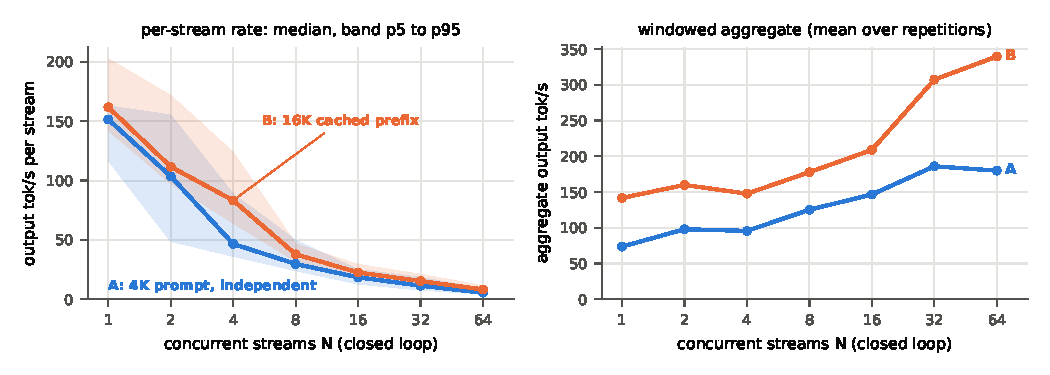
\includegraphics[width=\linewidth]{figures/generated/controlled_E8}
\caption{Controlled E8 sweep (pod 1, \texttt{gen30} plan). Left: output rate per stream against the number of
concurrent users $N$, median with a p5 to p95 band over the requests of each level (warm requests and errors excluded,
repetitions pooled). Right: windowed aggregate output rate, mean over repetitions (two in B, and in A two only at
$N=1$, where the mean includes a slow first repetition). A: independent 4K-token code prompts. B: 16K-token cached
prefix.}
\label{fig:ctl-E8}
\end{figure}

When every user brings a new prompt, reading competes with writing and the total stops growing earlier, at
\dv{ctl.E8.main.A-code-4k.closed:8.agg_mean} tokens/s with eight users, \dv{ctl.E8.main.A-code-4k.closed:32.agg_mean}
with 32 and \dv{ctl.E8.main.A-code-4k.closed:64.agg_mean} with 64, while TTFT p95 rises to
\dv{ctl.E8.main.A-code-4k.closed:64.ttft_p95}\,s. Reading alone, one prompt at a time, takes
\dv{ctl.E8.probes.prefill-4096.closed:1.ttft_p50}, \dv{ctl.E8.probes.prefill-16384.closed:1.ttft_p50} and
\dv{ctl.E8.probes.prefill-65536.closed:1.ttft_p50}\,s for 4K, 16K and 64K tokens. Two caveats apply to this sweep. The
cached-prefix scenario has two repetitions per level, but the unique-prompt scenario has two only for one user. In its
second repetition a single client-side disconnect among eight requests tripped the pre-registered stop rule and ended
the sweep, a rule we have since made less sensitive. That one-user level also pools a slow first repetition (TTFT p95
\dv{ctl.E8.main.A-code-4k.closed:1.ttft_p95}\,s), so its aggregate is not a steady-state rate.

% Generated by hostoffload.analysis.pipeline. Do not edit.
\begin{table}[t]
\centering
\small
\begin{fittable}{tab:ctl-E8}
\begin{tabular}{llrrrrrrrr}
\toprule
scenario & load & $n$ & TTFT p50 & p95 & p99 & TPOT p50 & p95 & E2E p50 & p99 \\
\midrule
\addlinespace\multicolumn{10}{l}{\textit{main}, pod 1} \\
A-code-4k & closed:1 & 16 & 0.65 & 9.44 & 25.81 & 6.6 & 9.6 & 2.3 & 29.4 \\
A-code-4k & closed:2 & 8 & 0.68 & 1.31 & 1.31 & 9.8 & 20.8 & 3.5 & 6.4 \\
A-code-4k & closed:4 & 8 & 0.65 & 1.28 & 1.30 & 22.1 & 27.7 & 6.3 & 8.4 \\
A-code-4k & closed:8 & 16 & 1.13 & 2.26 & 2.26 & 33.6 & 41.5 & 9.4 & 12.6 \\
A-code-4k & closed:16 & 32 & 2.65 & 5.40 & 5.47 & 54.2 & 78.1 & 17.2 & 25.0 \\
A-code-4k & closed:32 & 64 & 3.57 & 10.15 & 10.38 & 87.5 & 130.0 & 26.5 & 39.9 \\
A-code-4k & closed:64 & 128 & 4.77 & 27.29 & 28.85 & 182.2 & 235.2 & 53.2 & 83.4 \\
B-prefix-16k & closed:1 & 16 & 0.30 & 0.31 & 0.32 & 6.2 & 7.0 & 1.9 & 2.2 \\
B-prefix-16k & closed:2 & 16 & 0.42 & 0.45 & 0.46 & 9.0 & 10.3 & 2.6 & 3.1 \\
B-prefix-16k & closed:4 & 16 & 0.44 & 0.58 & 0.68 & 12.0 & 15.6 & 3.5 & 4.7 \\
B-prefix-16k & closed:8 & 32 & 0.52 & 0.82 & 0.89 & 26.4 & 31.4 & 7.3 & 8.9 \\
B-prefix-16k & closed:16 & 64 & 0.78 & 1.07 & 1.16 & 44.3 & 55.9 & 12.1 & 16.3 \\
B-prefix-16k & closed:32 & 128 & 1.19 & 1.59 & 1.66 & 65.3 & 87.7 & 17.9 & 24.9 \\
B-prefix-16k & closed:64 & 256 & 1.67 & 2.03 & 2.18 & 121.1 & 153.0 & 32.3 & 44.1 \\
\addlinespace\multicolumn{10}{l}{\textit{probes}, pod 1} \\
decode & closed:1 & 4 & 0.19 & 0.21 & 0.21 & 6.7 & 7.9 & 3.6 & 4.3 \\
decode & closed:8 & 8 & 0.85 & 0.85 & 0.85 & 21.2 & 22.6 & 11.7 & 12.3 \\
decode & closed:32 & 32 & 15.15 & 15.32 & 15.32 & 59.5 & 66.2 & 45.3 & 49.0 \\
prefill-4096 & closed:1 & 3 & 0.63 & 0.66 & 0.66 & 0.0 & 0.0 & 0.6 & 0.7 \\
prefill-16384 & closed:1 & 3 & 1.56 & 1.60 & 1.60 & 0.0 & 0.0 & 1.6 & 1.6 \\
prefill-65536 & closed:1 & 3 & 6.19 & 6.39 & 6.41 & 0.0 & 0.0 & 6.2 & 6.4 \\
\bottomrule
\end{tabular}
\end{fittable}
\caption{Controlled: Main benchmark of the measured stack as run (gen30 plan; scenarios A and B at N = 1 to 64, two repetitions in B and in A only at N = 1; prefill and decode probes, one repetition). Part 1 of 2, per-request latency: time to first token (TTFT, s), time per output token (TPOT, ms) and end-to-end time (E2E, s), with requests pooled over repetitions. Rows are grouped by variant and pod session (Table~\ref{tab:pod-hardware}). Throughput and SLOs of the same load points: Table~\ref{tab:ctl-E8-thr}.}
\label{tab:ctl-E8}
\end{table}
\begin{table}[t]
\centering
\small
\begin{fittable}{tab:ctl-E8-thr}
\begin{tabular}{llrrrrl}
\toprule
scenario & load & R & $n$ & aggregate tok/s & CV\% & SLO \\
\midrule
\addlinespace\multicolumn{7}{l}{\textit{main}, pod 1} \\
A-code-4k & closed:1 & 2 & 16 & 73.6 & 68.9 & - \\
A-code-4k & closed:2 & 1 & 8 & 97.9 & - & i,r,l \\
A-code-4k & closed:4 & 1 & 8 & 95.6 & - & i,r,l \\
A-code-4k & closed:8 & 1 & 16 & 125.2 & - & r,l \\
A-code-4k & closed:16 & 1 & 32 & 146.5 & - & r \\
A-code-4k & closed:32 & 1 & 64 & 186.0 & - & - \\
A-code-4k & closed:64 & 1 & 128 & 179.9 & - & - \\
B-prefix-16k & closed:1 & 2 & 16 & 141.7 & 5.2 & i,r,l \\
B-prefix-16k & closed:2 & 2 & 16 & 159.9 & 0.8 & i,r,l \\
B-prefix-16k & closed:4 & 2 & 16 & 147.7 & 4.6 & i,r,l \\
B-prefix-16k & closed:8 & 2 & 32 & 177.7 & 5.7 & i,r,l \\
B-prefix-16k & closed:16 & 2 & 64 & 208.9 & 7.2 & r,l \\
B-prefix-16k & closed:32 & 2 & 128 & 307.2 & 4.3 & r \\
B-prefix-16k & closed:64 & 2 & 256 & 339.5 & 7.5 & - \\
\addlinespace\multicolumn{7}{l}{\textit{probes}, pod 1} \\
decode & closed:1 & 1 & 4 & 133.2 & - & i,r,l \\
decode & closed:8 & 1 & 8 & 333.3 & - & i,r,l \\
decode & closed:32 & 1 & 32 & 334.5 & - & - \\
prefill-4096 & closed:1 & 1 & 3 & 1.6 & - & - \\
prefill-16384 & closed:1 & 1 & 3 & 0.6 & - & - \\
prefill-65536 & closed:1 & 1 & 3 & 0.2 & - & - \\
\bottomrule
\end{tabular}
\end{fittable}
\caption{Controlled: Main benchmark of the measured stack as run (gen30 plan; scenarios A and B at N = 1 to 64, two repetitions in B and in A only at N = 1; prefill and decode probes, one repetition). Part 2 of 2, throughput and objectives. R: repetitions at that point; aggregate: mean over repetitions of the windowed output rate (tokens/s), CV its coefficient of variation across repetitions (- for a single repetition); SLO: initials of the pre-registered SLOs met in every repetition. Latency of the same load points: Table~\ref{tab:ctl-E8}.}
\label{tab:ctl-E8-thr}
\end{table}


The same trade sets the cost of a token. At \dv{price.2xpro6000.usd_h}\,USD per pod-hour, with the whole hour charged
to output tokens (an upper bound for output that says nothing about input), one million output tokens cost
\dv{ctl.E8.main.B-prefix-16k.closed:1.usd_per_m_out}\,USD with one user on the cached prefix and
\dv{ctl.E8.main.B-prefix-16k.closed:64.usd_per_m_out}\,USD with 64, and \dv{ctl.E8.main.A-code-4k.closed:8.usd_per_m_out}
and \dv{ctl.E8.main.A-code-4k.closed:32.usd_per_m_out}\,USD at eight and 32 users with unique prompts, so the
cheapest tokens are those written when each stream is slowest. We registered three service-level objectives before
the controlled runs (Section~\ref{sec:method}). With the cached prefix the interactive one (TTFT p95 up to 2\,s and
TPOT p95 up to 50\,ms) holds in every repetition up to eight users and the relaxed one up to 32. With unique prompts
the interactive objective holds from two to four users and the relaxed one from two to 16, and the one-user level
misses both because of its slow first repetition (SLO column of Table~\ref{tab:ctl-E8-thr}). For coding agents the useful unit is the number of streams that stay fast, which is the
subject of Section~\ref{sec:agent}.\label{sec:cost}

\paragraph{Long prompts cost reading (E12).}
Coding agents work with long contexts, so we pushed the prompt to the context limit of
\dv{ctl.kv.max_len} tokens on the second pod. Reading grows as expected. A fresh prompt of 128K tokens waits
\dv{ctl.E12.long.prefill-long-131072.closed:1.ttft_p50}\,s for its first token, and one of 260,000 tokens
\dv{ctl.E12.long.prefill-long-260000.closed:1.ttft_p50}\,s. Writing by a single request hardly notices the length. It
takes \dv{ctl.E12.long.decode-128k.closed:1.tpot_p50_ms}\,ms per token after a 128K-token prompt and
\dv{ctl.E12.long.decode-256k.closed:1.tpot_p50_ms}\,ms after a 256K-token one, against
\dv{ctl.E3.gen30-session2.A-code-4k.closed:1.tpot_p50_ms}\,ms after a 4K-token prompt on the same pod. That changes
when several long requests write at once, at \dv{ctl.E12.long.decode-128k.closed:4.tpot_p50_ms}\,ms per token with
four 128K requests and \dv{ctl.E12.long.decode-256k.closed:2.tpot_p50_ms}\,ms with two of 256K.
Figure~\ref{fig:read-write} puts the two phases side by side: reading climbs with the length of the prompt, and
writing stays flat.

\begin{figure}[t]
\centering
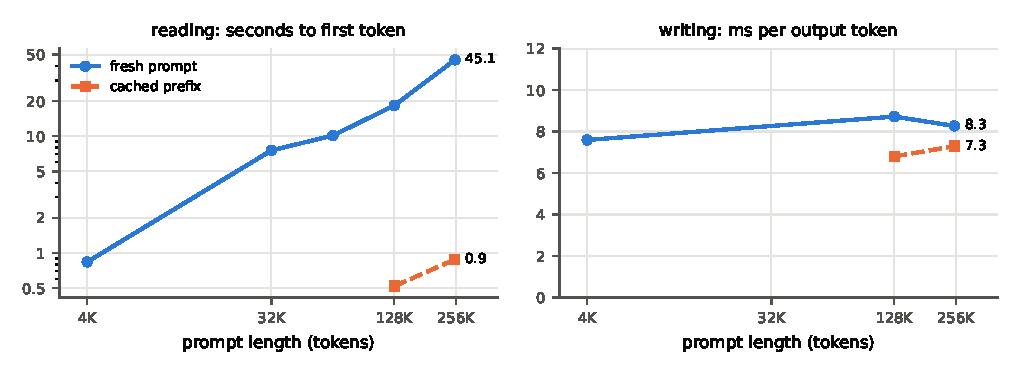
\includegraphics[width=\linewidth]{figures/generated/read_write_length.pdf}
\caption{Reading against writing for one request on pod~2 (one repetition, median of 2 to 8 requests per point).
Left: time to first token against prompt length, for fresh prompts and for prompts behind a cached prefix (log
scales). Right: time per output token against prompt length. The 4K point is the E3 \texttt{gen30} run on the same
pod, and the other points are E12. Values from Tables~\ref{tab:ctl-E12} and~\ref{tab:ctl-E3}, lengths from
\datafile{experiments/workloads/long_context.yaml}.}
\label{fig:read-write}
\end{figure}

When the long context is shared and cached, as for agents working on one large codebase, the reading is paid once.
With a 128K-token cached prefix, TTFT p95 is \dv{ctl.E12.long.B-prefix-128k.closed:8.ttft_p95}\,s at eight users, and
with 256K tokens it is \dv{ctl.E12.long.B-prefix-256k.closed:4.ttft_p95}\,s at four users with
\dv{ctl.E12.long.B-prefix-256k.closed:4.tpot_p50_ms}\,ms per token. A long context therefore stays interactive once it
has been read, and the expensive case is many users with different long prompts, where reading sets the limit. vLLM's
estimate of how many full-length requests fit in the KV cache (\dv{ctl.kv.max_concurrency}) is why E12 ran distinct
long prompts only up to four at 128K and two at 256K, and Section~\ref{sec:agent} shows that the estimate is
conservative. Each point is one repetition, on the second pod, which was slower than the first, and without a quality
check at these lengths (Tables~\ref{tab:ctl-E12} and~\ref{tab:ctl-E12-thr}).

% Generated by hostoffload.analysis.pipeline. Do not edit.
\begin{table}[t]
\centering
\small
\begin{fittable}{tab:ctl-E12}
\begin{tabular}{llrrrrrrrr}
\toprule
scenario & load & $n$ & TTFT p50 & p95 & p99 & TPOT p50 & p95 & E2E p50 & p99 \\
\midrule
\addlinespace\multicolumn{10}{l}{\textit{long}, pod 2} \\
B-prefix-128k & closed:1 & 4 & 0.52 & 0.57 & 0.57 & 6.8 & 7.2 & 2.3 & 2.3 \\
B-prefix-128k & closed:2 & 4 & 0.54 & 0.68 & 0.70 & 8.7 & 11.1 & 2.8 & 3.4 \\
B-prefix-128k & closed:4 & 8 & 0.66 & 1.19 & 1.33 & 13.2 & 19.2 & 4.0 & 6.1 \\
B-prefix-128k & closed:8 & 16 & 0.79 & 1.18 & 1.24 & 38.3 & 46.7 & 10.5 & 12.7 \\
B-prefix-256k & closed:1 & 4 & 0.88 & 0.89 & 0.89 & 7.3 & 7.5 & 2.7 & 2.8 \\
B-prefix-256k & closed:2 & 4 & 0.93 & 0.94 & 0.94 & 9.9 & 10.8 & 3.5 & 3.7 \\
B-prefix-256k & closed:4 & 8 & 1.26 & 1.66 & 1.70 & 16.6 & 19.6 & 5.4 & 6.1 \\
decode-128k & closed:1 & 2 & 22.45 & 25.13 & 25.36 & 8.7 & 10.4 & 26.9 & 28.9 \\
decode-128k & closed:2 & 2 & 27.10 & 34.05 & 34.67 & 29.1 & 43.1 & 42.0 & 42.2 \\
decode-128k & closed:4 & 4 & 48.20 & 71.72 & 73.77 & 68.4 & 118.4 & 83.7 & 84.2 \\
decode-256k & closed:1 & 2 & 44.75 & 47.79 & 48.06 & 8.3 & 9.3 & 49.0 & 52.9 \\
decode-256k & closed:2 & 2 & 58.74 & 75.79 & 77.30 & 48.2 & 81.8 & 83.3 & 83.5 \\
prefill-long-32768 & closed:1 & 3 & 7.57 & 10.75 & 11.04 & 0.0 & 0.0 & 7.6 & 11.0 \\
prefill-long-65536 & closed:1 & 3 & 10.14 & 14.91 & 15.34 & 0.0 & 0.0 & 10.1 & 15.3 \\
prefill-long-131072 & closed:1 & 3 & 18.33 & 18.46 & 18.48 & 0.0 & 0.0 & 18.3 & 18.5 \\
prefill-long-260000 & closed:1 & 3 & 45.07 & 58.68 & 59.89 & 0.0 & 0.0 & 45.1 & 59.9 \\
\bottomrule
\end{tabular}
\end{fittable}
\caption{Controlled: Long context at 128K and 256K tokens as run (pod 2; prefill, decode and cached shared prefix, one repetition). Part 1 of 2, per-request latency: time to first token (TTFT, s), time per output token (TPOT, ms) and end-to-end time (E2E, s), with requests pooled over repetitions. Rows are grouped by variant and pod session (Table~\ref{tab:pod-hardware}). Throughput and SLOs of the same load points: Table~\ref{tab:ctl-E12-thr}.}
\label{tab:ctl-E12}
\end{table}
\begin{table}[t]
\centering
\small
\begin{fittable}{tab:ctl-E12-thr}
\begin{tabular}{llrrrrl}
\toprule
scenario & load & R & $n$ & aggregate tok/s & CV\% & SLO \\
\midrule
\addlinespace\multicolumn{7}{l}{\textit{long}, pod 2} \\
B-prefix-128k & closed:1 & 1 & 4 & 111.0 & - & i,r,l \\
B-prefix-128k & closed:2 & 1 & 4 & 90.9 & - & i,r,l \\
B-prefix-128k & closed:4 & 1 & 8 & 115.3 & - & i,r,l \\
B-prefix-128k & closed:8 & 1 & 16 & 126.8 & - & i,r,l \\
B-prefix-256k & closed:1 & 1 & 4 & 92.5 & - & i,r,l \\
B-prefix-256k & closed:2 & 1 & 4 & 91.8 & - & i,r,l \\
B-prefix-256k & closed:4 & 1 & 8 & 177.9 & - & i,r,l \\
decode-128k & closed:1 & 1 & 2 & 20.6 & - & - \\
decode-128k & closed:2 & 1 & 2 & 24.3 & - & - \\
decode-128k & closed:4 & 1 & 4 & 24.3 & - & - \\
decode-256k & closed:1 & 1 & 2 & 11.4 & - & - \\
decode-256k & closed:2 & 1 & 2 & 12.3 & - & - \\
prefill-long-32768 & closed:1 & 1 & 3 & 0.1 & - & - \\
prefill-long-65536 & closed:1 & 1 & 3 & 0.1 & - & - \\
prefill-long-131072 & closed:1 & 1 & 3 & 0.1 & - & - \\
prefill-long-260000 & closed:1 & 1 & 3 & 0.0 & - & - \\
\bottomrule
\end{tabular}
\end{fittable}
\caption{Controlled: Long context at 128K and 256K tokens as run (pod 2; prefill, decode and cached shared prefix, one repetition). Part 2 of 2, throughput and objectives. R: repetitions at that point; aggregate: mean over repetitions of the windowed output rate (tokens/s), CV its coefficient of variation across repetitions (- for a single repetition); SLO: initials of the pre-registered SLOs met in every repetition. Latency of the same load points: Table~\ref{tab:ctl-E12}.}
\label{tab:ctl-E12-thr}
\end{table}


\paragraph{The size of the back room (E3).}
Putting more experts in the back room costs speed. Moving from the \texttt{gen30} plan to the union of its cold set
and that of the recipe's \texttt{agent30} plan lowers the total output with unique code prompts from
\dv{ctl.E3.gen30.A-code-4k.closed:1.agg_mean} to \dv{ctl.E3.union-gen30-agent30.A-code-4k.closed:1.agg_mean}
tokens/s with one user, from \dv{ctl.E3.gen30.A-code-4k.closed:8.agg_mean} to
\dv{ctl.E3.union-gen30-agent30.A-code-4k.closed:8.agg_mean} with eight and from
\dv{ctl.E3.gen30.A-code-4k.closed:32.agg_mean} to \dv{ctl.E3.union-gen30-agent30.A-code-4k.closed:32.agg_mean} with 32
(Table~\ref{tab:ctl-E3-thr}, one repetition per point, two boots). The decode scenario of the larger share is missing,
because the load generator stopped on a client-side disconnect while the server kept serving.

We also wanted to compare Diffbot's per-expert machinery with the zero-copy offload that upstream vLLM already ships,
at the same host bytes. We could not compare speed, because upstream's offload does not serve this model on these
pins. With the KV block size of 64 that the measured stack uses, it fails at initialization, since the FlashInfer
sparse-attention backend for DeepSeek-V4.1 accepts only blocks of 128. With 128 the server boots, and the engine dies
on the first request, because DeepGEMM's attention kernel asserts a block of 32 or 64
(\datafile{data/controlled/E3-host-share/uva-equal-gen30/} and \datafile{data/controlled/E3-host-share/uva-equal-gen30-bs128/}). Two kernels on the
same attention path accept different block sizes, and with the recipe's runtime hooks (sfxnz's, edited by Diffbot)
the stack serves with blocks of 64. On this hardware and these pins the hooks are needed to serve at all, so whether
the per-expert split is also faster than upstream's offload remains open.

% Generated by hostoffload.analysis.pipeline. Do not edit.
\begin{table}[t]
\centering
\small
\begin{fittable}{tab:ctl-E3}
\begin{tabular}{llrrrrrrrr}
\toprule
scenario & load & $n$ & TTFT p50 & p95 & p99 & TPOT p50 & p95 & E2E p50 & p99 \\
\midrule
\addlinespace\multicolumn{10}{l}{\textit{gen30}, pod 1} \\
A-code-4k & closed:1 & 8 & 0.64 & 0.66 & 0.66 & 6.5 & 7.0 & 2.3 & 2.4 \\
A-code-4k & closed:8 & 16 & 1.05 & 1.70 & 1.72 & 31.3 & 35.4 & 8.8 & 10.9 \\
A-code-4k & closed:32 & 64 & 3.38 & 9.05 & 9.56 & 86.6 & 111.1 & 26.0 & 36.9 \\
decode & closed:1 & 4 & 0.21 & 0.21 & 0.21 & 6.0 & 6.4 & 3.3 & 3.5 \\
decode & closed:8 & 8 & 0.83 & 0.84 & 0.84 & 21.3 & 22.1 & 11.6 & 12.2 \\
decode & closed:32 & 32 & 1.33 & 1.33 & 1.46 & 60.2 & 67.5 & 32.1 & 36.4 \\
\addlinespace\multicolumn{10}{l}{\textit{gen30-session2}, pod 2} \\
A-code-4k & closed:1 & 8 & 0.84 & 10.89 & 15.21 & 7.6 & 7.9 & 2.8 & 17.1 \\
A-code-4k & closed:8 & 16 & 1.65 & 2.81 & 2.87 & 43.3 & 55.2 & 13.2 & 16.0 \\
A-code-4k & closed:32 & 64 & 4.88 & 17.75 & 18.41 & 130.9 & 180.1 & 38.5 & 61.9 \\
decode & closed:1 & 4 & 0.22 & 0.24 & 0.24 & 7.4 & 9.4 & 4.0 & 5.1 \\
decode & closed:8 & 8 & 0.94 & 0.94 & 0.94 & 29.4 & 30.4 & 15.7 & 16.6 \\
decode & closed:32 & 32 & 12.33 & 12.33 & 12.50 & 77.2 & 90.3 & 51.5 & 58.6 \\
\addlinespace\multicolumn{10}{l}{\textit{union-gen30-agent30}, pod 1} \\
A-code-4k & closed:1 & 8 & 0.88 & 1.76 & 2.12 & 8.7 & 9.7 & 3.2 & 4.3 \\
A-code-4k & closed:8 & 16 & 1.92 & 2.77 & 2.77 & 42.0 & 54.8 & 12.6 & 16.5 \\
A-code-4k & closed:32 & 64 & 4.51 & 13.03 & 13.65 & 121.2 & 165.2 & 36.3 & 53.7 \\
\bottomrule
\end{tabular}
\end{fittable}
\caption{Controlled: Host share as run (rung (c) of the ablation ladder): the gen30 plan against the union of the gen30 and agent30 cold sets on pod 1, and the gen30 subset repeated on pod 2 (variant gen30-session2), one repetition per point. Part 1 of 2, per-request latency: time to first token (TTFT, s), time per output token (TPOT, ms) and end-to-end time (E2E, s), with requests pooled over repetitions. Rows are grouped by variant and pod session (Table~\ref{tab:pod-hardware}). Throughput and SLOs of the same load points: Table~\ref{tab:ctl-E3-thr}.}
\label{tab:ctl-E3}
\end{table}
\begin{table}[t]
\centering
\small
\begin{fittable}{tab:ctl-E3-thr}
\begin{tabular}{llrrrrl}
\toprule
scenario & load & R & $n$ & aggregate tok/s & CV\% & SLO \\
\midrule
\addlinespace\multicolumn{7}{l}{\textit{gen30}, pod 1} \\
A-code-4k & closed:1 & 1 & 8 & 112.1 & - & i,r,l \\
A-code-4k & closed:8 & 1 & 16 & 146.6 & - & i,r,l \\
A-code-4k & closed:32 & 1 & 64 & 197.9 & - & - \\
decode & closed:1 & 1 & 4 & 159.7 & - & i,r,l \\
decode & closed:8 & 1 & 8 & 335.5 & - & i,r,l \\
decode & closed:32 & 1 & 32 & 446.9 & - & r \\
\addlinespace\multicolumn{7}{l}{\textit{gen30-session2}, pod 2} \\
A-code-4k & closed:1 & 1 & 8 & 51.4 & - & - \\
A-code-4k & closed:8 & 1 & 16 & 102.2 & - & r,l \\
A-code-4k & closed:32 & 1 & 64 & 125.4 & - & - \\
decode & closed:1 & 1 & 4 & 132.2 & - & i,r,l \\
decode & closed:8 & 1 & 8 & 246.3 & - & i,r,l \\
decode & closed:32 & 1 & 32 & 278.3 & - & - \\
\addlinespace\multicolumn{7}{l}{\textit{union-gen30-agent30}, pod 1} \\
A-code-4k & closed:1 & 1 & 8 & 76.6 & - & i,r,l \\
A-code-4k & closed:8 & 1 & 16 & 115.9 & - & r,l \\
A-code-4k & closed:32 & 1 & 64 & 139.7 & - & - \\
\bottomrule
\end{tabular}
\end{fittable}
\caption{Controlled: Host share as run (rung (c) of the ablation ladder): the gen30 plan against the union of the gen30 and agent30 cold sets on pod 1, and the gen30 subset repeated on pod 2 (variant gen30-session2), one repetition per point. Part 2 of 2, throughput and objectives. R: repetitions at that point; aggregate: mean over repetitions of the windowed output rate (tokens/s), CV its coefficient of variation across repetitions (- for a single repetition); SLO: initials of the pre-registered SLOs met in every repetition. Latency of the same load points: Table~\ref{tab:ctl-E3}.}
\label{tab:ctl-E3-thr}
\end{table}


\paragraph{The host matters (E3 on two pods).}
The second session repeated the \texttt{gen30} subset of E3, with the same stack, plan and workload, on another host.
It was slower at every point. The median time per token was \dv{ctl.pod.cross.A.N1.tpot_ratio} to
\dv{ctl.pod.cross.A.N32.tpot_ratio} times pod~1's, and the total output \dv{ctl.pod.cross.decode.N32.agg_ratio} to
\dv{ctl.pod.cross.decode.N1.agg_ratio} times, except for one user with unique prompts
(\dv{ctl.pod.cross.A.N1.agg_ratio}), where a single request with a TTFT of \dv{ctl.pod.cross.A.N1.pod2.ttft_max}\,s
explains most of the gap (Table~\ref{tab:cross-pod}). Both hosts have the same GPU model, driver and PCIe Gen5 x16
links (Table~\ref{tab:pod-hardware}). One difference shows up in a single word of the topology table that
\texttt{nvidia-smi topo -m} prints. Between the two GPUs, pod~1 reports \texttt{\dv{ctl.pod.s1.gpu_link}} and pod~2
reports \texttt{\dv{ctl.pod.s2.gpu_link}}. On pod~1 both GPUs hang from the same CPU socket (NUMA node), while on
pod~2 each sits on a different socket, so tensor-parallel traffic and reads from host memory cross the link between
sockets. That is a plausible cause, but the CPUs also differ (\dv{ctl.pod.s1.cpu} against \dv{ctl.pod.s2.cpu}), both
servers had served other workloads on the same boot before this subset, and one repetition per pod cannot separate
these causes from each other or from variation between boots. What the data show is that the host a cloud pod lands
on matters as much as most settings we varied, and that numbers from different pods are not directly comparable.

% Generated by hostoffload.analysis.pipeline. Do not edit.
\begin{table}[t]
\centering
\small
\begin{fittable}{tab:cross-pod}
\begin{tabular}{lrrrrrrr}
\toprule
scenario & $N$ & aggr. pod 1 & pod 2 & ratio & TPOT p50 pod 1 & pod 2 & ratio \\
\midrule
A: 4K prompt & 1 & 112 & 51 & 0.46 & 6.5 & 7.6 & 1.17 \\
 & 8 & 147 & 102 & 0.70 & 31.3 & 43.3 & 1.38 \\
 & 32 & 198 & 125 & 0.63 & 86.6 & 130.9 & 1.51 \\
decode & 1 & 160 & 132 & 0.83 & 6.0 & 7.4 & 1.23 \\
 & 8 & 335 & 246 & 0.73 & 21.3 & 29.4 & 1.38 \\
 & 32 & 447 & 278 & 0.62 & 60.2 & 77.2 & 1.28 \\
\bottomrule
\end{tabular}
\end{fittable}
\par\smallskip\parbox{0.95\linewidth}{\footnotesize\raggedright Sources: \datafile{data/controlled/E3-host-share/gen30/20261006T203206Z}, \datafile{data/controlled/E3-host-share/gen30-session2/20261007T063646Z}. Levels whose slowest request had a TTFT above 10 s: A: 4K prompt $N=1$ on pod 2, 16.3 s; A: 4K prompt $N=32$ on pod 2, 18.4 s; decode $N=32$ on pod 2, 12.6 s.}
\caption{The same E3 subset workload (\texttt{gen30} plan, identical stack and workload file, one repetition) on pod 1 and pod 2: windowed aggregate output rate (tok/s) and median TPOT (ms) per load point, and the ratio pod 2 / pod 1. With one repetition per pod the ratio mixes the host difference with run-to-run and boot-to-boot variance.}
\label{tab:cross-pod}
\end{table}


\paragraph{Traffic on the bus and speculation.}
The PCIe receive rate, summed over both GPUs, peaked at \dv{ctl.pcie.E8.B.N32.gbs}\,GB/s in E8, and DSpark, which
proposes \dv{ctl.spec.k} draft tokens per step that the model then verifies, gained a request
\dv{ctl.spec.E8.A.accept_len} tokens per verification step on unique code prompts. Section~\ref{sec:bytes} gives both
in full, with the caveats on the PCIe counters and on speculation, which was always on and is therefore not separated
from the offload in any number above. The protocol of every experiment in this section is in
Section~\ref{sec:method}, and the hardware of the three pods in Section~\ref{sec:setup}.
